\subsection{Cantilevers}

\begin{figure}
  \begin{center}
  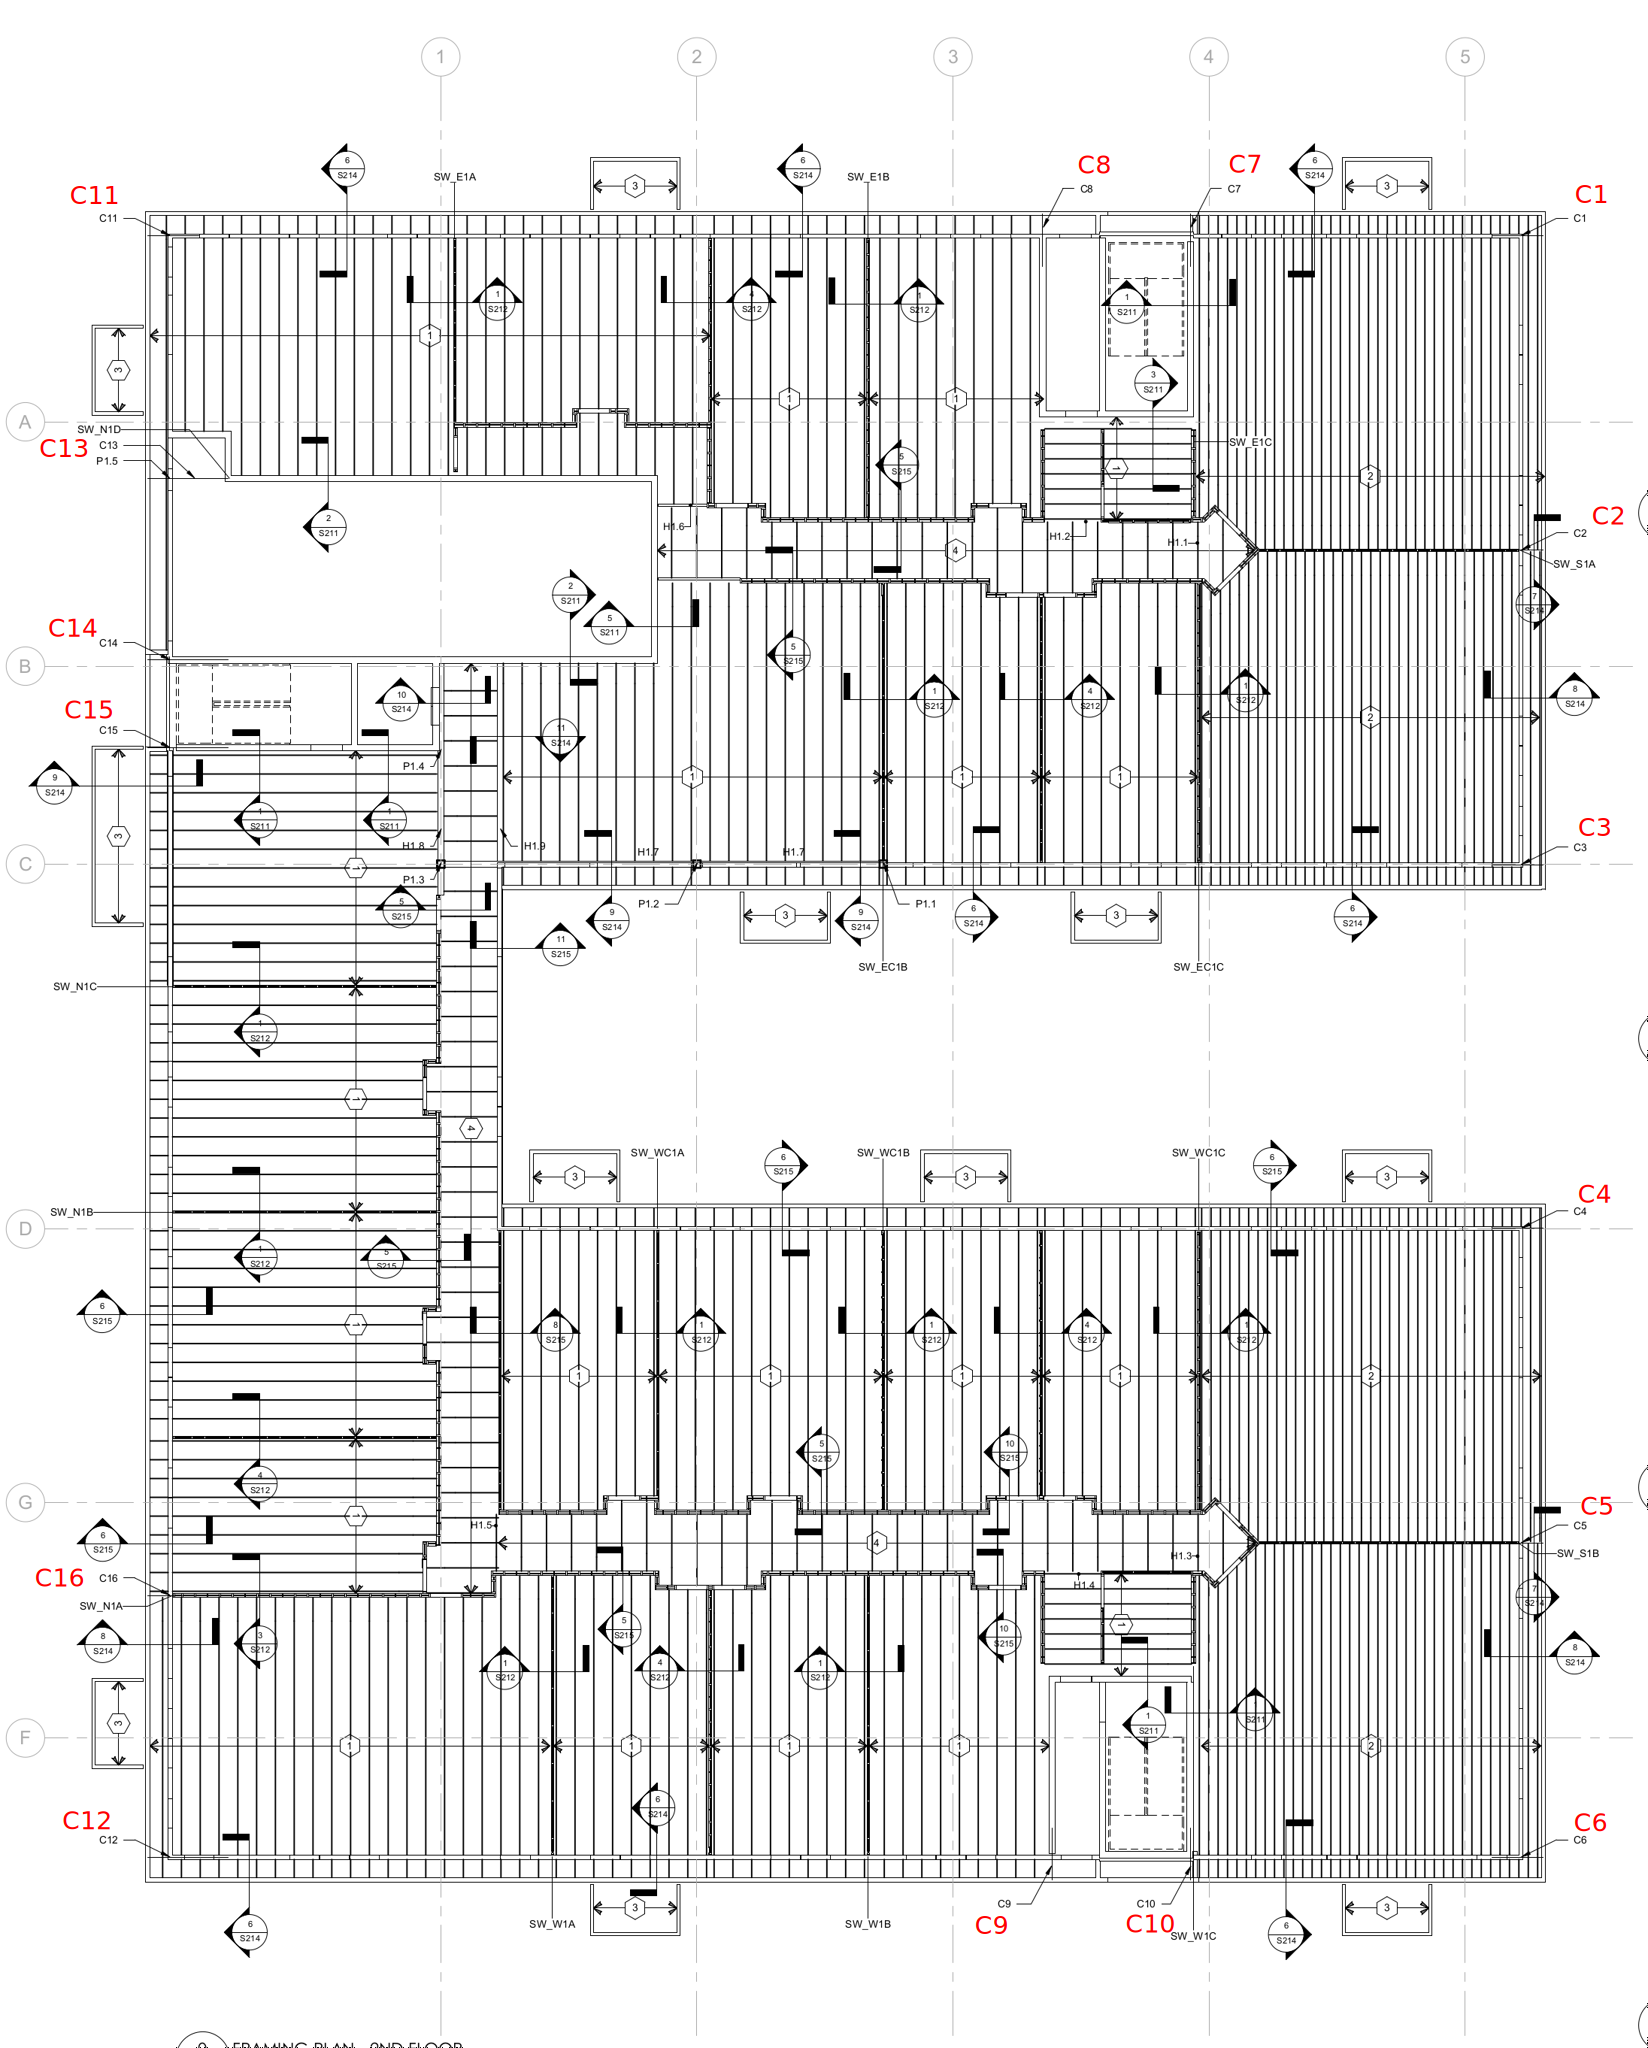
\includegraphics[width=120mm]{figures/cantilevers/cantilevers_key_plan}
  \end{center}
  \caption{Second floor cantilevers key plan.}\label{fg_2nd_floor_cantilevers_key_plan}
\end{figure}

\subsubsection{Cantilevers C1, C3, C4, C6, C7 and C8}

\paragraph{Loads.}

\begin{itemize}
\item Load from trusses (three trusses at 12 inches): 13.21 kN/truss
\item Facade weight: 25.76 kN
\item Total load: 65.41 kN
\end{itemize}

\paragraph{Internal forces.}

\noindent Maximum induced moment:

\begin{equation}
  M_{max}= 37.98\ kN m
\end{equation}

\noindent Maximum induced shear:

\begin{equation}
  V_{max}= 65.41\ kN
\end{equation}

\paragraph{Structural bending check.}

\noindent LSL 1.55E 5.25x14'' design resisting moment:

\begin{equation}
  M'_s= 44.89\ kN m
\end{equation}

\noindent Structural bending check: $M'_s = 44.89 > 37.98 = M_{max} \implies OK$

\paragraph{Structural shear check.}

\noindent LSL 1.55E 5.25x14'' design resisting shear:
\begin{equation}
  V'_s= 89.36\ kN
\end{equation}

\noindent Structural shear check: $V'_s = 89.36 > 65.41 = V_{max} \implies OK$

\paragraph{Bending stiffness.}
The deflection obtained under total load is:

\begin{equation}
  \Delta_{TL}= 1.88\ mm= \frac{L}{506} < \frac{L}{360} \implies OK
\end{equation}

\subsubsection{Cantilevers C2 and C5}

\paragraph{Loads.}

\begin{itemize}
\item Load from trusses (2x3 trusses at 12 inches): 13 kN/truss
\item Facade weight: 51.55 kN
\item Total load: 129.25 kN
\end{itemize}

\paragraph{Internal forces.}

\noindent Maximum induced moment:

\begin{equation}
  M_{max}= 63.79\ kN m
\end{equation}

\noindent Maximum induced shear:

\begin{equation}
  V_{max}= 129.25\ kN
\end{equation}

\paragraph{Structural bending check.}

\noindent (2) LSL 1.55E 5.25x14'' design resisting moment:

\begin{equation}
  M'_s= 65.88\ kN m
\end{equation}

\noindent Structural bending check: $M'_s = 65.88 > 63.79 = M_{max} \implies OK$

\paragraph{Structural shear check.}

\noindent (2) LSL 1.55E 5.25x14'' design resisting shear:
\begin{equation}
  V'_s= 151.60\ kN
\end{equation}

\noindent Structural shear check: $V'_s = 151.60 > 129.25 = V_{max} \implies OK$

\paragraph{Bending stiffness.}
The deflection obtained under total load is:

\begin{equation}
  \Delta_{TL}= 1.95\ mm= \frac{L}{442} < \frac{L}{360} \implies OK
\end{equation}

\subsubsection{Cantilever C9}

\paragraph{Loads.}

\begin{itemize}
\item Floor load: 16.25 kN
\item Facade weight: 36.37 kN
\item Total load: 52.62 kN
\end{itemize}

\paragraph{Internal forces.}

\noindent Maximum induced moment:

\begin{equation}
  M_{max}= 49.99\ kN m
\end{equation}

\noindent Maximum induced shear:

\begin{equation}
  V_{max}= 52.62\ kN
\end{equation}

\paragraph{Structural bending check.}

\noindent LSL 1.55E 5.25x18'' design resisting moment:

\begin{equation}
  M'_s= 72.00\ kN m
\end{equation}

\noindent Structural bending check: $M'_s = 72.00 > 49.99 = M_{max} \implies OK$

\paragraph{Structural shear check.}

\noindent LSL 1.55E 5.25x18'' design resisting shear:
\begin{equation}
  V'_s= 114.90\ kN
\end{equation}

\noindent Structural shear check: $V'_s = 114.90 > 52.62 = V_{max} \implies OK$

\paragraph{Bending stiffness.}
The deflection obtained under total load is:

\begin{equation}
  \Delta_{TL}= 1.5\ mm= \frac{L}{717} < \frac{L}{360} \implies OK
\end{equation}

\subsubsection{Cantilever C10}

\paragraph{Loads.}

\begin{itemize}
\item Floor load: 10.84 kN
\item Facade weight: 24.25 kN
\item Total load: 35.08 kN
\end{itemize}

\paragraph{Internal forces.}

\noindent Maximum induced moment:

\begin{equation}
  M_{max}= 33.33\ kN m
\end{equation}

\noindent Maximum induced shear:

\begin{equation}
  V_{max}= 35.08\ kN
\end{equation}

\paragraph{Structural bending check.}

\noindent LSL 1.55E 3.5x18'' design resisting moment:

\begin{equation}
  M'_s= 48.00\ kN m
\end{equation}

\noindent Structural bending check: $M'_s = 48.00 > 33.33 = M_{max} \implies OK$

\paragraph{Structural shear check.}

\noindent LSL 1.55E 3.5x18'' design resisting shear:
\begin{equation}
  V'_s= 76.60\ kN
\end{equation}

\noindent Structural shear check: $V'_s = 76.60 > 35.08 = V_{max} \implies OK$

\paragraph{Bending stiffness.}
The deflection obtained under total load is:

\begin{equation}
  \Delta_{TL}= 1.33\ mm= \frac{L}{717} < \frac{L}{360} \implies OK
\end{equation}

\begin{table}
  \begin{center}
  \includegraphics[width=120mm]{figures/cantilevers/cantilever_schedule}
  \end{center}
  \caption{Cantilever schedule.}\label{fg_2nd_floor_cantilevers_schedule}
\end{table}
